\documentclass[11pt,class=report,crop=false]{standalone}
\usepackage{exo7hilisit}

\begin{document}

%%%%%%%%%%%%%%%%%%%%%%%%%%%%%%%%%%%%%%%%%%%%%%%%%%%%%%%%%%%%%%%%%%%%%%
%%%%%%%%%%%%%%%%%%%%%%%%%%%%%%%%%%%%%%%%%%%%%%%%%%%%%%%%%%%%%%%%%%%%%%


\entete{Hilisit}{Capacité mathématiques}

\titre{Logique et raisonnements -- Partie 2 : Ensembles} 

\encadre{
	\emph{Savoir.}
	\begin{itemize}[label=$\square$]
		\item Maîtriser le vocabulaire des ensembles : élément, inclusion, complémentaire, union, intersection.
        \item Maîtriser le vocabulaire des fonctions : image, antécédent, bijection.
        
	\end{itemize}
	\emph{Savoir-faire.}
	\begin{itemize}[label=$\square$]
		\item Savoir calculer des unions, intersections, complémentaires d'ensembles.
        \item Savoir déterminer un domaine de définition.
        \item Savoir calculer une composition et montrer qu'une fonction est bijective.
	\end{itemize}
}



\bigskip

%-----------------------------------------
\subsection*{Ensembles}

\begin{itemize}
  \item Un \textbf{ensemble} est une collection d'objets distincts que l'on appelle des \textbf{éléments}. On note la liste des éléments qui définissent un ensemble en utilisant des accolades : $\big\{ \, . \, . \, . \big\}$.
  
  \item On peut définir un ensemble soit par \emph{extension}, en énumérant l'ensemble de ses éléments. Ainsi l'ensemble des nombres apparaissant sur les faces d'un dé est $\{1 , 2 , 3 , 4 , 5 , 6\}$.
  
  \item On peut également définir un ensemble par \emph{compréhension} en décrivant ses éléments par une ou plusieurs propriétés qui les caractérisent. Dans ce cadre, l'ensemble des entiers pairs peut s'écrire : $\{2k \mid k \in \Zz\}$.
  
  \item L'ensemble qui ne comporte aucun élément est appelé \textbf{l'ensemble vide} ; on le note $\varnothing$. Un ensemble qui ne comporte qu'un unique élément est appelé un \emph{singleton}. Une \emph{paire} est un ensemble de deux éléments distincts.
  
  \item Si un élément $e$ appartient à l'ensemble $E$, on note : $e \in E$ (on dit aussi que $E$ \emph{contient} $e$). Dans le cas contraire, on écrit : $e \notin E$.
\end{itemize}


%-----------------------------------------
\subsection*{Inclusion, complémentaire}

\begin{itemize}
  \item \textbf{Inclusion.} Si $A$ et $B$ sont deux ensembles, l'écriture  $A \subset B$ indique que "\emph{$A$ est inclus dans $B$}", ce qui signifie que tout élément de $A$ appartient aussi à $B$. On dit aussi que $A$ est une \emph{partie} ou un \emph{sous-ensemble} de $B$.

  \item \textbf{Égalité.} Deux ensemble $A$ et $B$ sont égaux s'ils ont exactement les mêmes éléments. D'un point de vue logique, cela équivaut à dire qu'ils sont mutuellement inclus l'un dans l'autre : 
  $$ A = B \iff (\; A \subset B \; \text{ et } \; B \subset A \;)$$
   
  \item \textbf{Complémentaire.} Si $A$ est une partie d'un ensemble $E$, on définit le \emph{complémentaire de A}, noté $E \setminus A$ (ou encore $\overline{A}$), comme l'ensemble des éléments de $E$ qui n'appartiennent pas à $A$ : 
  $$E \setminus A  :=  \{x \in E \mid x \notin A\}$$
\end{itemize}

On représente souvent les opérations sur les ensembles par de petits schémas appelés des \emph{diagrammes de Venn}. En voici deux exemples pour l'inclusion et le complémentaire de deux ensembles.
 
\begin{center}
   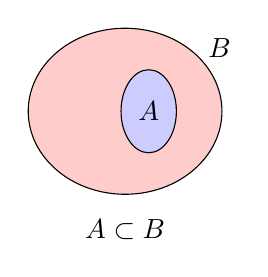
\begin{tikzpicture}
   \fill[fill=red!20,draw=black] (0,0) ellipse (35pt and 30pt);
   \fill[fill=blue!20,draw=black] (0.3,0) ellipse (10pt and 15pt);
   
   \node at (0.3,0) {$A$};
   \node at (1.2,0.8) {$B$};
   \node at (0,-1.5) {$A \subset B$};
   \end{tikzpicture} 
\qquad\qquad    
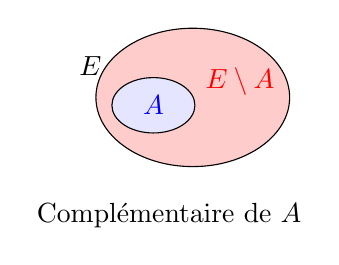
\begin{tikzpicture}
\fill[fill=red!20,draw=black] (0.3,0)  ellipse (35pt and 25pt);
\fill[fill=blue!10,draw=black] (-0.2,-0.1)  ellipse (15pt and 10pt);
\node[blue] at (-0.2,-0.1) {$A$};
\node[red] at (0.9,0.2) {$E \setminus A$};
\node at (-1,0.4) {$E$};
\node at (0,-1.5) {Complémentaire de $A$};
\end{tikzpicture} 
\end{center}


\emph{Exemple.}
Soit $E = \{ 1 , 2 , 3 , 4 , 5 \}$ et $A = \{ 2 , 5 \}$.
\begin{itemize}
    \item L'ensemble $E$ contient $5$ éléments ; $A$ contient $2$ éléments.
    \item Tout élément de $A$ appartient à $E$, donc $A \subset E$.
    \item Le complémentaire de $A$ dans $E$ est $E \setminus A = \{ 1 , 3 , 4  \}$.
\end{itemize}

\emph{Autres exemples.}
\begin{itemize}
    \item L'ensemble des nombres pairs $P=\{2k \mid k \in \Zz\}$ est un sous-ensemble des entiers relatifs $\Zz$. Son complémentaire dans $\Zz$ est : $\Zz \setminus P=\{ 2k+1 \mid k\in \Zz\}$. Il s'agit bien sûr des entiers impairs !
    \item $\Rr\setminus\{0\}$, que l'on note souvent $\Rr^\star$, est l'ensemble des nombres réels non nuls.
\end{itemize}

Les ensembles que nous connaissons et utilisons le plus fréquemment sont les ensembles de nombres. Il y a ainsi par exemple  :
\begin{itemize}
    \item L'ensemble des nombres premiers $\mathcal{P}$

    \item L'ensemble des nombres entiers naturels $\Nn$

    \item L'ensemble des nombres entiers relatifs $\Zz$

    \item L'ensemble des nombres rationnels $\Qq := \{ \frac p q \mid p\in \Zz, \; q \in \Nn^\star \}$

    \item L'ensemble des nombres réels $\Rr$

    \item L'ensemble des nombres complexes $\Cc$
\end{itemize}
On a d'ailleurs les inclusions : 
$$\mathcal{P} \subset \Nn \subset \Zz \subset \Qq \subset \Rr \subset \Cc.$$


%-----------------------------------------
\subsection*{Union, intersection}


\begin{itemize}
    \item \textbf{L'union de $A$ et $B$} est l'ensemble des éléments qui sont soit dans $A$, soit dans $B$ (et éventuellement dans les deux à la fois). On la note : \boldmath $A \cup B$\unboldmath \ définie par $A \cup B =  \{ x \mid  x \in A \text{ ou } x \in B \}$.

    \item \textbf{L'intersection de $A$ et $B$} est l'ensemble des éléments qui sont à la fois dans $A$ et dans $B$. On la note : \boldmath $A \cap B$\unboldmath \ définie par $A \cap B = \{x \mid  x \in A \text{ et } x \in B \}$.
    
    \item Si $A \cap B = \varnothing$, on dit que les ensembles $A$ et $B$ sont \textbf{disjoints}.
\end{itemize}

\begin{center}
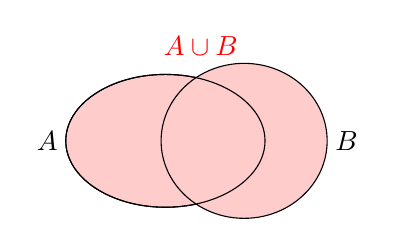
\begin{tikzpicture}

\fill[fill=red!20,draw=black] (0,0) ellipse (36pt and 24pt);
\fill[fill=red!20,draw=black] (1,0) ellipse (30pt and 28pt);
\draw (0,0) ellipse (36pt and 24pt);

\node at (-1.5,0) {$A$};
\node at (2.3,0) {$B$};
\node[red] at (0.45,1.2) {$A\cup B$};
\end{tikzpicture}
\qquad\qquad
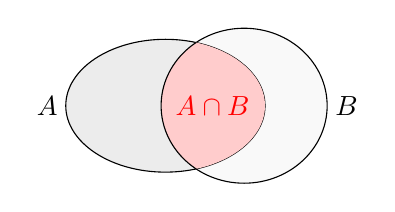
\begin{tikzpicture}

\fill[fill=gray!5,draw=black] (1,0) ellipse (30pt and 28pt);

\fill[fill=gray!15,draw=black]  (0,0) ellipse (36pt and 24pt);

\begin{scope}
  \clip (0,0) ellipse (36pt and 24pt);
  \fill[fill=red!20,draw=black] (1,0) ellipse (30pt and 28pt);
\end{scope}


\node at (-1.5,0) {$A$};
\node at (2.3,0) {$B$};
\node[red] at (0.6,0) {$A\cap B$};
\end{tikzpicture}
\qquad\qquad
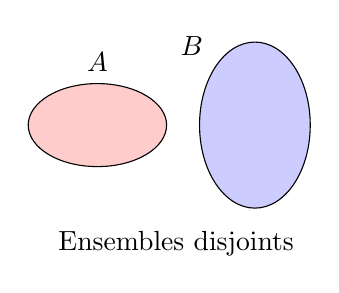
\begin{tikzpicture}
\fill[fill=red!20,draw=black] (0,0) ellipse (25pt and 15pt);
\fill[fill=blue!20,draw=black] (2,0) ellipse (20pt and 30pt);

\node at (0,0.8) {$A$};
\node at (1.2,1) {$B$};
\node at (1,-1.5) {Ensembles disjoints};
\end{tikzpicture}

\end{center}



\emph{Exemple.}
Si $A = \{ 1 , 2 , 3 \}$ et $B = \{ 2 , 4 \}$, alors on a :
    $$A \cup B = \{ 1 , 2 , 3 , 4  \} \qquad  \qquad A \cap B = \{ 2 \}.$$
    
    
%-----------------------------------------
\subsection*{Fonctions}

\begin{itemize}
  \item Une \textbf{fonction} (ou une \textbf{application}) d'un ensemble $E$ vers un ensemble $F$, est la donnée pour chaque élément $x$ de $E$ d'un unique élément $y$ de $F$. On écrit alors cela : $f(x)=y$. L'élément $y$ s'appelle l'\textbf{image} de $x$, et l'élément $x$ est un \textbf{antécédent} de $y$.

\begin{center}
\shorthandoff{:!}
\begin{tikzpicture}[scale=1.2]
\node (x) at (0,0.5) {};
\node (fx) at (2.3,0.5) {};
\node (y) at (-0.3,0.1) {};
\node (fy) at (2.4,0) {};
\node (z) at (0.3,-0.6) {};
\node (fz) at (2.8,-0.7){};
\node (w) at (-0.35,-0.5) {};
\node (xx) at (0.2,-0.2) {};

\draw[thick] (0,0) ellipse (24pt and 30pt);
\node at (-29pt,0) {$E$};
\fill (x) circle (2pt);
\fill (y) circle (2pt);
\fill[myred] (z) circle (2pt);
\fill[myred] (w) circle (2pt);
\fill[myred] (xx) circle (2pt);

\draw[thick] (2.5,0) ellipse (23pt and 35pt);
\node at (2.5cm+30pt,0) {$F$};
\fill (fx) circle (2pt);
\fill (fy) circle (2pt);
\fill[myred] (fz) circle (2pt);
\fill (2.8,0.1) circle (2pt);
\node at (1.25,40pt) {$f$};

\path[->, thick] (x) edge[out=60,in=120] (fx);
\path[->, thick] (y) edge[out=30,in=150] (fy);
\path[->, thick] (z) edge[out=0,in=190] (fz);
\path[->, thick] (w) edge[out=-40,in=-110] (fz);
\path[->, thick] (xx) edge[out=10,in=150] (fz);

\node[right] at (fz) {$y$};
\node[left] at (w) {$x_1$};
\node[left] at (z) {$x_2$};
\node[left] at (xx) {$x_3$};
\end{tikzpicture}
\shorthandon{:!}
\qquad\qquad\qquad
\begin{tikzpicture}[scale=1.3]

\draw[->,>=latex, black, very thin] (-0.7,0) -- (3,0) node[above] {$x$};
\draw[->,>=latex, black, very thin] (0,-0.5) -- (0,2.5) node[left] {$y$};

\draw[domain=-0.7:2.9,black,thick,smooth] plot (\x,{0.6+0.4*\x+0.6*cos(2*\x r)});

%	\draw[myred,very thick] (-0.25,0)--(2.5,0) node[midway,below] {$E$};
%	\draw[myred,very thick] (0,0.3)--(0,1.83) node[near end,left] {$F$};

\draw[dashed] (-0.42,0) -- (-0.42,0.85);
\draw[dashed] (0.9,0) -- (0.9,0.85);
\draw[dashed] (1.85,0) -- (1.85,0.85);

\draw[dashed] (-0.4,0.85) -- (1.9,0.85);

\fill[myred]  (-0.45,0) circle (2pt) node[below] {$x_1$};
\fill[myred]  (0.9,0) circle (2pt) node[below] {$x_2$};
\fill[myred]  (1.85,0) circle (2pt) node[below] {$x_3$};

\fill[myred]  (0,0.85) circle (2pt) node[below right] {$y$};

\end{tikzpicture}
  
\end{center}
  
  \item On note cette application "$ f  :  E \longrightarrow F$, $x \longmapsto f(x)$".
  
  \item L'ensemble $E$ s'appelle le \textbf{domaine de définition} de $f$ (il est parfois noté $\mathcal{D}_f$).
  
  \item Ce sera souvent à vous de déterminer le domaine de définition (le plus grand possible). 
  Par exemple l'expression $f(x)=\sqrt x$ définit une fonction $f : [0,+\infty[ \to \Rr$.
  En effet pour avoir le droit d'écrire $\sqrt{x}$ il faut que $x$ soit positif ou nul.
\end{itemize}
  

\emph{Exercice.}
Déterminer les domaines de définition (dans $\Rr$) des fonctions définies par les expressions suivantes :
\begin{itemize}
    \item $f(x) = \frac{x-1}{x+1}$
    \item $f(x) = \sqrt{x+3}$   
    \item $f(x) = \ln(3x-7)$
    \item $f(x) = \sqrt{\frac1{x^2-2}}$    
\end{itemize}

%-----------------------------------------
\subsection*{Composition}

\textbf{Composition}
    Soient $E, F, G$ trois ensembles, et $f  :  E \longrightarrow F$, $g  :  F \longrightarrow G$ deux applications. Alors on peut définir la \textbf{composée} de $f$ par $g$, notée $g \circ f$, comme étant l'application :
    $g \circ f : E \to G$ définie par :
    \mybox{$(g\circ f) (x) = g \bigl( f(x) \bigr)$}

\begin{center}
\begin{tikzpicture}[node distance=2cm, every edge/.style={draw,thick,->}]
\node(E){$E$};
\node[right of=E](F){$F$};
\node[right of=F](G){$G$};
\draw (E) edge (F);\draw (E) edge[myred, bend left=45] node[above]{$f$} (F);
\draw (F) edge (G);\draw (F) edge[myred, bend left=45] node[above]{$g$} (G);
\draw (E) edge[myred, bend right] node[below]{$g\circ f$} (G);
\end{tikzpicture}
\end{center}

\medskip

\emph{Exemple.}
Soit $f : \Rr \to \Rr$ définie par $f(x) = x^2$ et soit $g : \Rr \to \Rr$ définie par $g(x) = \cos(2x+1)$, alors $g \circ f : \Rr \to \Rr$ est la fonction donnée par :
$$(g \circ f)(x) = g \bigl( f(x) \bigr) = g(x^2) = \cos(2x^2+1)$$

Attention $f \circ g$ est aussi définie mais est une toute autre application.
Son expression est donnée par :
$$(f \circ g)(x) = f \bigl( g(x) \bigr) = f\bigl( \cos(2x+1)\bigr) = \big( \cos(2x+1) \big)^2.$$

\medskip



\emph{Exemple.}
Soit $f : \Rr^{\star}_+ \to \Rr^{\star}_+$ définie par $f(x) = \frac{1}{x}$
et $g : \Rr^{\star}_+ \to \Rr$ définie par $g(x) = \frac{x-2}{x+3}$
(rappel : $\Rr^{\star}_+ =  ]0 , +\infty[$).
Alors
$$(g \circ f)(x)
= g \bigl( f(x) \bigr)
= g \biggl( \frac{1}{x} \biggr) 
= \frac{ \frac1x - 2}{ \frac 1x +3}\underbrace{\quad = \quad }_{\times x > 0}\frac{1-2x}{1+3x}$$



%-----------------------------------------
\subsection*{Bijection}

\begin{itemize}
    \item \textbf{Bijection.} 
On dit que l'application $f :  E \to F$ est \textbf{bijective} si chaque élément de $F$ possède un antécédent par $f$, et que cet antécédent est de plus unique.
Dans ce cas, l'application $f$ établit une correspondance parfaite entre les éléments de $E$ et les éléments de $F$.

\begin{center}
\shorthandoff{:!}
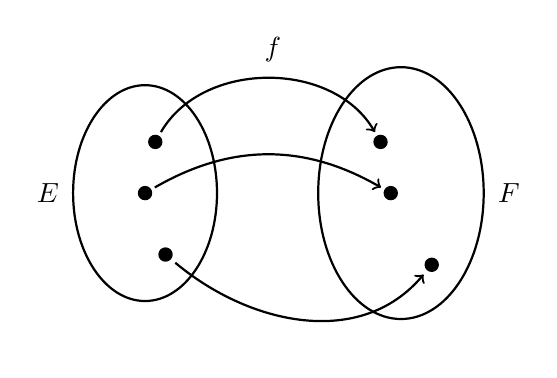
\begin{tikzpicture}[scale=1.3]

\node (x) at (0.1,0.5) {};
\node (fx) at (2.3,0.5) {};
\node (y) at (0.,0) {};
\node (fy) at (2.4,0) {};
\node (z) at (0.2,-0.6) {};
\node (fz) at (2.8,-0.7) {};

\draw[thick] (0,0) ellipse (20pt and 30pt);
\node at (-27pt,0) {$E$};
\fill (x) circle (2pt);
\fill (y) circle (2pt);
\fill (z) circle (2pt);

\draw[thick] (2.5,0) ellipse (23pt and 35pt);
\node at (2.5cm+30pt,0) {$F$};
\fill (fx) circle (2pt);
\fill (fy) circle (2pt);
\fill (fz) circle (2pt);

\node at (1.25,40pt) {$f$};

\path[->, thick] (x) edge[out=60,in=120] (fx);
\path[->, thick] (y) edge[out=30,in=150] (fy);
\path[->, thick] (z) edge[out=-40,in=-130] (fz);

\end{tikzpicture}
\shorthandon{:!}
\qquad\qquad\qquad
\begin{tikzpicture}[scale=1.3]

\draw[->,>=latex, black, very thin] (-0.5,0) -- (3,0) node[above] {$x$};
\draw[->,>=latex, black, very thin] (0.5,-0.5) -- (0.5,2.5) node[left] {$y$};

\draw[domain=-0.25:2.5,black,thick] plot (\x,{0.1*(\x+2)*(\x+2)});

\draw[dashed] (-0.25,0) -- (-0.25,0.306) -- (0.5,0.306);
\draw[dashed] (2.5,0) -- (2.5,2.025) -- (0.5,2.025);

\draw[myred,very thick] (-0.25,0)--(2.5,0) node[midway,below] {$E$};
\draw[myred,very thick] (0.5,0.306)--(0.5,2.025) node[midway,left] {$F$};

\end{tikzpicture}
\end{center}

    \item Si $f : E \to F$ est bijective, alors l'application $g : F \to E$ qui à tout élément de $y$ de $F$ associe son unique antécédent $x$ par $f$ dans $E$ est bien définie et est également bijective. Elle est notée $f^{-1}$ et s'appelle la \textbf{bijection réciproque} de $f$.

    \item On a alors $(f^{-1} \circ f)(x) = x$ (pour tout $x \in E$)
    et aussi $(f\circ f^{-1})(y) = y$ (pour tout $y \in F$).

    \item Exemple. Soit $f : [0,+\infty[ \to [0,+\infty[$, $x \mapsto x^2$. Sa bijection réciproque est 
    la fonction racine carrée : $f^{-1} : [0,+\infty[ \to [0,+\infty[$, $x \mapsto \sqrt{x}$.
    On a bien $(\sqrt x)^2 = x$ et $\sqrt{x^2} = x$, pour tout $x\ge0$.

    
    \item Exponentielle et logarithme sont bijections réciproques l'une de l'autre :
    $\exp(\ln(x)) = x$ (pour tout $x>0$) et $\ln(\exp(x)) = x$ (pour tout $x\in\Rr$).
    
\end{itemize}    

\end{document}
